\begin{figure}[h]
\centering
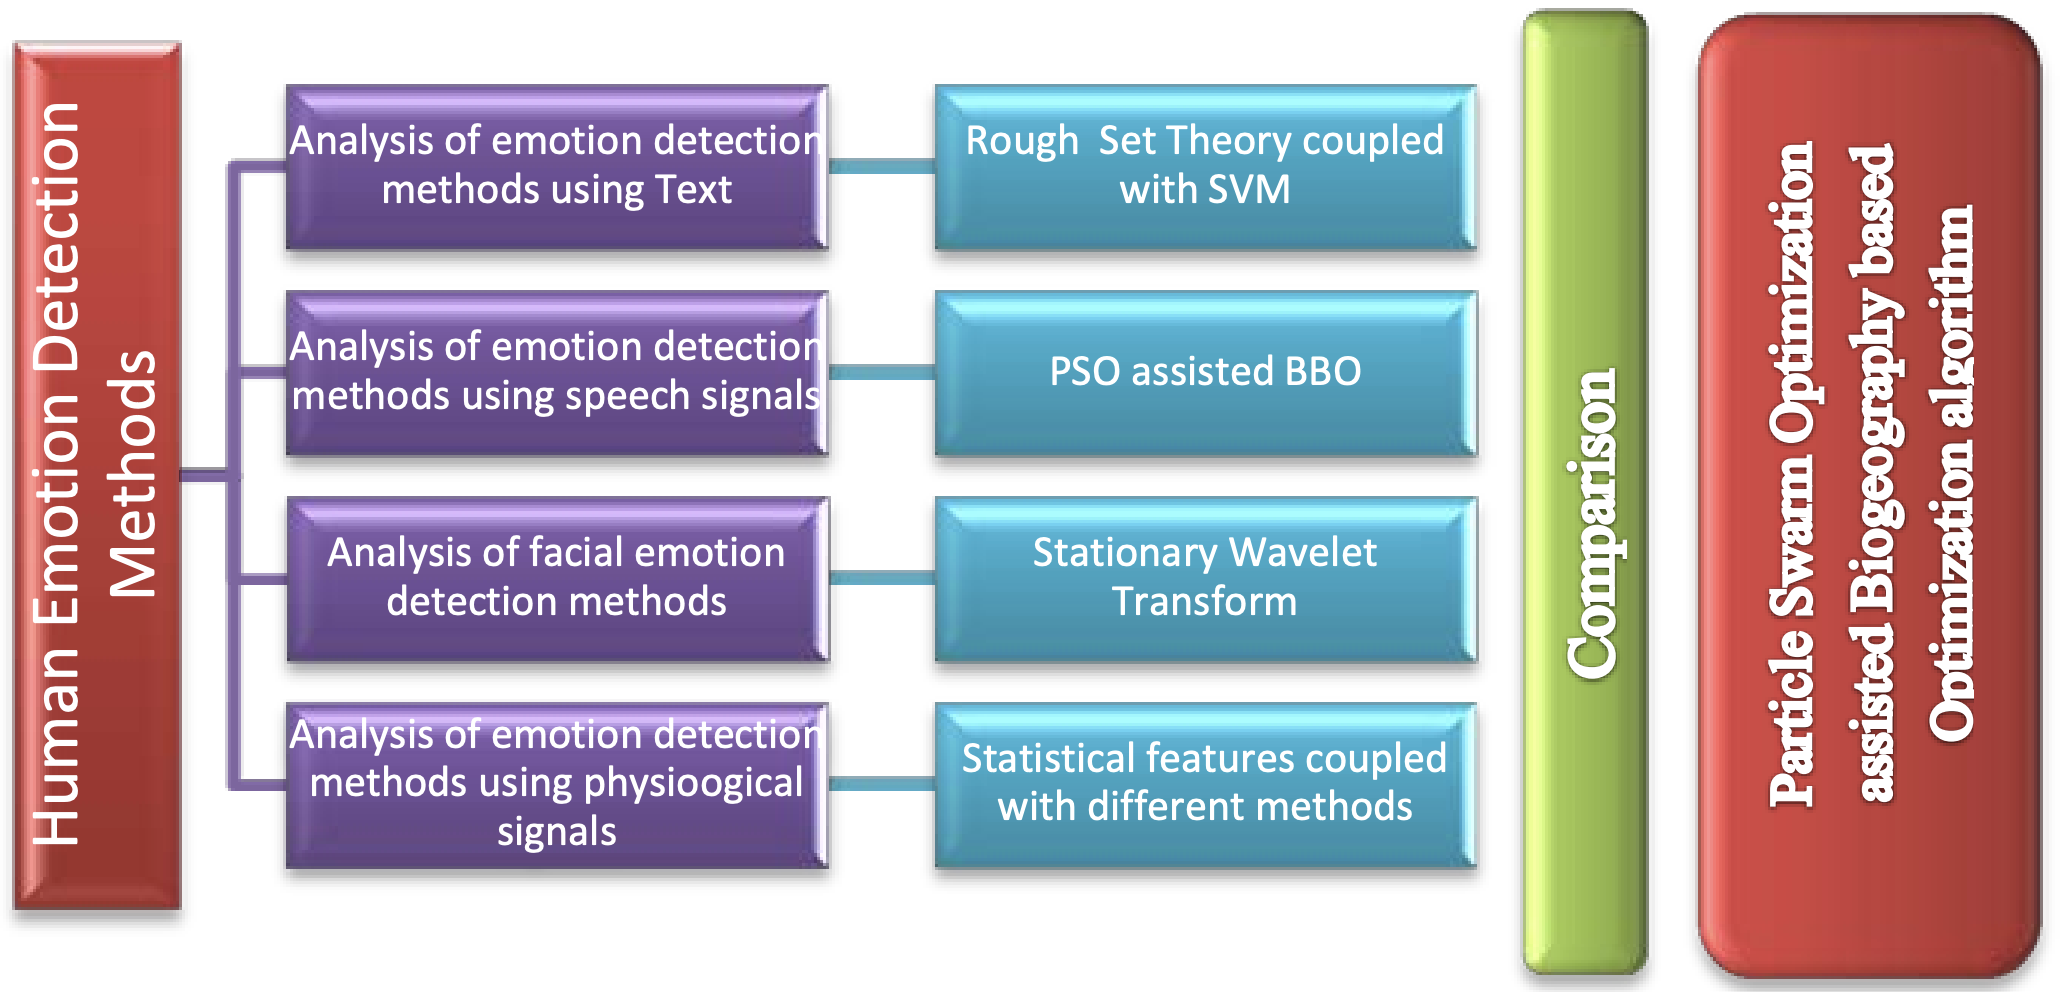
\includegraphics[width=1\textwidth]{images/Emotion-detection-survey.png}
\caption{Survey on Emotional Detection. \cite{survey}}\label{fig:survey}
\end{figure}

\noindent The current work on emotional recognition is an active and rapidly developing field with many applications as already touched upon in chapter \ref{chap:introduction}. Like figure \ref{fig:survey} shows, there are many possibilities to approach this. Continuing, we will focus on \acrshort{fer} and \acrshort{ser}.\\

\noindent \acrshort{fer} is an important area of research that has many applications in \acrshort{hci} and other fields. \acrfull{cnn} have emerged as a promising approach for \acrshort{fer}, but there are numerous factors that can impact their performance. As of today, there are multiple state-of-the-art \acrshort{cnn}-based \acrshort{fer} methods that differ in their architecture, preprocessing, and training/test protocols, of which \cite{pramerdorfer2016facial} analyzed six.

\noindent Especially recognizing facial expressions under naturalistic conditions is still an unsolved problem and represents a great challenge. One way to improve \acrshort{fer} performance is to overcome the bottleneck of using comparatively basic CNN architectures. A collection of modern \acrshort{cnn} has achieved a FER2013 \cite{FER2013} test accuracy of 75.2\%, outperforming previous works without requiring auxiliary training data or face registration \cite{pramerdorfer2016facial}.

\noindent In the area of \acrshort{ser} the research is ongoing. Also, in the specific branch of \acrshort{hci} \acrshort{cnn} are commonly used for feature extraction and classification in \acrshort{ser}. Besides, \acrfull{rnn} (especially Gated Recurrent Unit architectures) are also effective methods for emotion recognition through speech. In this case the highest accuracy scored was 97.47\% was \cite{GRU}.

\noindent It is also interesting to have a look at the transformer-based models, which recently were used for \acrshort{ser} with promising results \cite{transform}. \acrshort{ser} under realistic conditions presents several challenges, including the variability in speech patterns and background noise.


% Quelle: https://www.mdpi.com/1424-8220/22/4/1414#:~:text=The%20data%20augmentation%20was%20used,average%20recognition%20accuracy%20of%2097.47%25.

%https://deepai.org/machine-learning-glossary-and-terms/gated-recurrent-unit

%https://www.nature.com/articles/s41598-022-12260-y